\section{Background}
The architecture and terms are instroduced in this section to serve the as basis for the further discussions. 
The figure~\ref{fig:architecture} demonstrates how a query is processed by a distributed query system. In this case, we use the Hadoop(HIive+Tez architecture) as an example.

\begin{figure}[t]
	\centering
	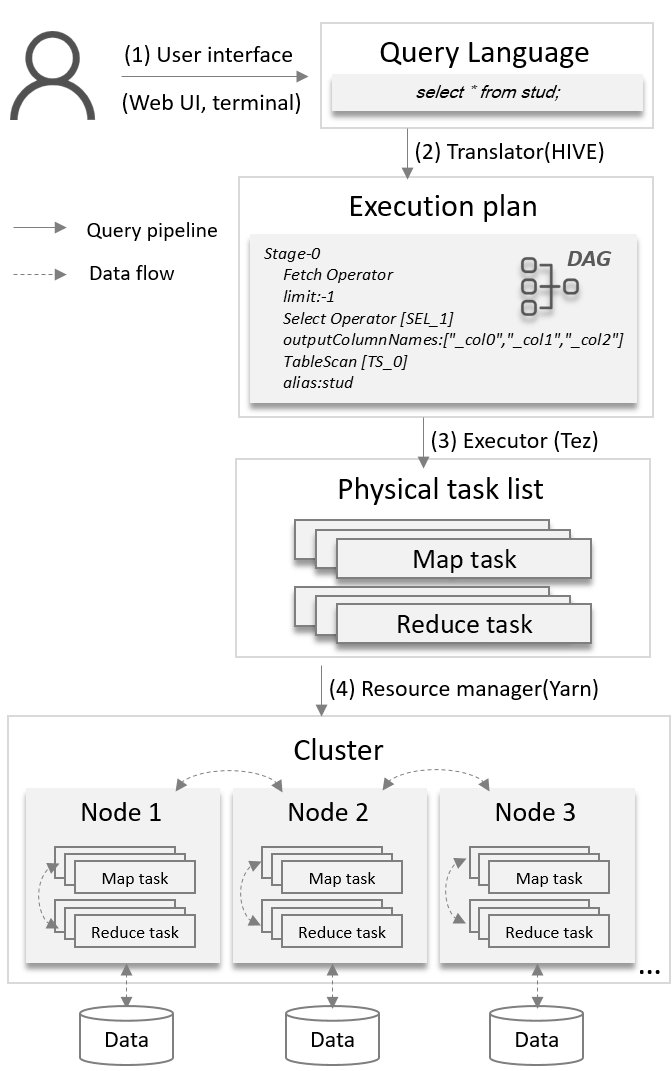
\includegraphics[width=0.40\textwidth]{figures/background/arc.png}
	\vspace{-3mm}
	\caption{Overview of Hive2.0 distributed query architecture.}
	\label{fig:architecture}
	\vspace{-3mm}
\end{figure}

When user issues a query (shown as Figure~\ref{fig:architecture}(1)) through the interface such as a web UI or SQL terminal, Hive optimizes it and translate it as the detail logic execution plan shown as Figure~\ref{fig:architecture}. The logic exaction plan may contains hundreds of lines of description, which usually describe the execution process as a Directed Acyclic Graph(DAG). The DAG includes two types of vertices: map vertex and reduce vertex. Each vertex contains a sequence of logic operators such as filter, aggregate, merge, etc. Moreover, there are edges to connect the verteices. The edges define the data movement between vertecies, the source vertices are the producers and the destinat vertices are the consumers.
Tez further generates the physical tasks according to the work flow of vertices and YARN dispatches these tasks on the Hadoop worker machines.  The task is the atomic process of the query. All tasks of the a specific vertex are dispatched to multiple machines and processed according to operators if the vertex.  